\documentclass[11pt,a4paper]{article}

\usepackage[utf8]{inputenc}
\usepackage[T1]{fontenc}
\usepackage[brazilian]{babel}
\usepackage{geometry}
\usepackage{graphicx}
\usepackage{booktabs}
\usepackage{amsmath}
\usepackage{float}
\usepackage{hyperref}

\geometry{margin=2.4cm}
\hypersetup{hidelinks}
\setlength{\parskip}{0.45em}
\setlength{\parindent}{0pt}

\title{DBO na entrada a partir de DQO e SST\\[0.3em]
\large Rede neural e validação cruzada}
\author{SoftSensor}
\date{16 de outubro de 2026}

\begin{document}
\maketitle

\section{Objetivo}

Estimar a demanda bioquímica de oxigênio na entrada da estação, \texttt{DBO-E}, com duas medições do mesmo ponto: a demanda química de oxigênio, \texttt{DQO-E}, e os sólidos em suspensão, \texttt{SS-E}. No arquivo, \texttt{SS-E} é o SST. A data não entra no modelo. Cada dia é uma observação independente.

\section{Dados}

O conjunto é o Water Treatment Plant, de Manel Poch (UCI, 1993). São 527 dias. Ficam 498 dias em que \texttt{DBO-E}, \texttt{DQO-E} e \texttt{SS-E} existem ao mesmo tempo; 29 dias saem por valor ausente. Não há interpolação. As unidades não estão documentadas na UCI, e os erros abaixo usam a mesma escala do arquivo.

\begin{table}[ht]
\centering
\caption{Entrada da planta nos 498 dias completos.}
\begin{tabular}{lrrrr}
\toprule
Variável & Mínimo & Mediana & Média (desvio) & Máximo \\
\midrule
DBO-E & 31 & 182,5 & 188,72 (62,28) & 438 \\
DQO-E & 81 & 397,5 & 405,36 (119,99) & 941 \\
SS-E  & 98 & 198 & 228,74 (139,12) & 2008 \\
\bottomrule
\end{tabular}
\end{table}

A correlação da DBO com a DQO é 0,565. Com o SST é 0,137. DQO e SST correlacionam 0,284 entre si. O máximo de \texttt{SS-E}, 2008, fica muito acima da mediana 198.

\section{Protocolo}

A amostra foi embaralhada e partida em 80\% de treino (398 dias) e 20\% de teste (100 dias), com \texttt{random\_state} 42. A DBO média é 188,14 no treino e 191,03 no teste.

A rede é um \texttt{MLPRegressor} com otimizador \texttt{lbfgs}, adequado a este tamanho de amostra. As entradas passam por um \texttt{StandardScaler} dentro de um \texttt{Pipeline}, ajustado só nas linhas de treino de cada partição. A validação cruzada tem 5 partições embaralhadas e escolhe a configuração de menor MAE. A grade cobre camadas \((8)\), \((16)\), \((32)\), \((16,8)\) e \((32,16)\), ativações ReLU e tangente hiperbólica, e regularização L2 \(\alpha \in \{10^{-4}, 10^{-3}, 10^{-2}, 10^{-1}\}\).

O teste é usado uma vez, depois da escolha. Duas referências, ajustadas no mesmo treino, situam o erro: a média da DBO de treino e uma regressão linear de \texttt{DQO-E} e \texttt{SS-E}.

\section{Resultados}

A validação cruzada escolhe uma camada de 8 neurônios, ReLU e \(\alpha = 10^{-4}\). O MAE nessa validação é 39,19, com desvio de 2,78 entre as partições. O ajuste final converge em 42 iterações. As oito melhores configurações ficam entre 39,19 e 39,99 de MAE. Trocar o tamanho da rede, a ativação ou \(\alpha\) mexe pouco no erro, e a rede menor permanece na frente.

\begin{table}[ht]
\centering
\caption{Erro no conjunto de teste (100 dias).}
\begin{tabular}{lrrr}
\toprule
Modelo & MAE & RMSE & \(R^{2}\) \\
\midrule
Média do treino & 44,11 & 56,83 & 0,00 \\
Regressão linear & 32,96 & 44,76 & 0,38 \\
MLP & 33,51 & 44,91 & 0,37 \\
\bottomrule
\end{tabular}
\end{table}

Na validação cruzada do treino, a regressão linear tem MAE 38,36 \(\pm\) 2,08, e o MLP tem 39,19 \(\pm\) 2,78. A ordem se repete no teste. O teste ficou um pouco mais fácil do que as partições de validação, para os dois modelos.

A reta ajustada nas unidades originais é
\begin{equation}
\widehat{\mathrm{DBO}} = 74{,}04 + 0{,}2872\,\mathrm{DQO} - 0{,}0127\,\mathrm{SST}.
\end{equation}
Num dia com DQO 400 e SST 200, a conta dá cerca de 186, perto da média da amostra. O coeficiente do SST é pequeno: cada unidade a mais de SST reduz a DBO prevista em 0,013.

Embaralhar a DQO no treino aumenta o MAE do MLP em 19,15 \(\pm\) 1,39. Embaralhar o SST aumenta o MAE em 0,10 \(\pm\) 0,08.

No teste, a previsão do MLP vai de 95,86 a 273,91. O resíduo médio (observado menos previsto) é 5,21. A mediana do erro absoluto é 22,07 e o percentil 90 é 79,31. Em 59 dos 100 dias o erro absoluto fica até 30; em 74 dias, até 50.

\begin{figure}[H]
\centering
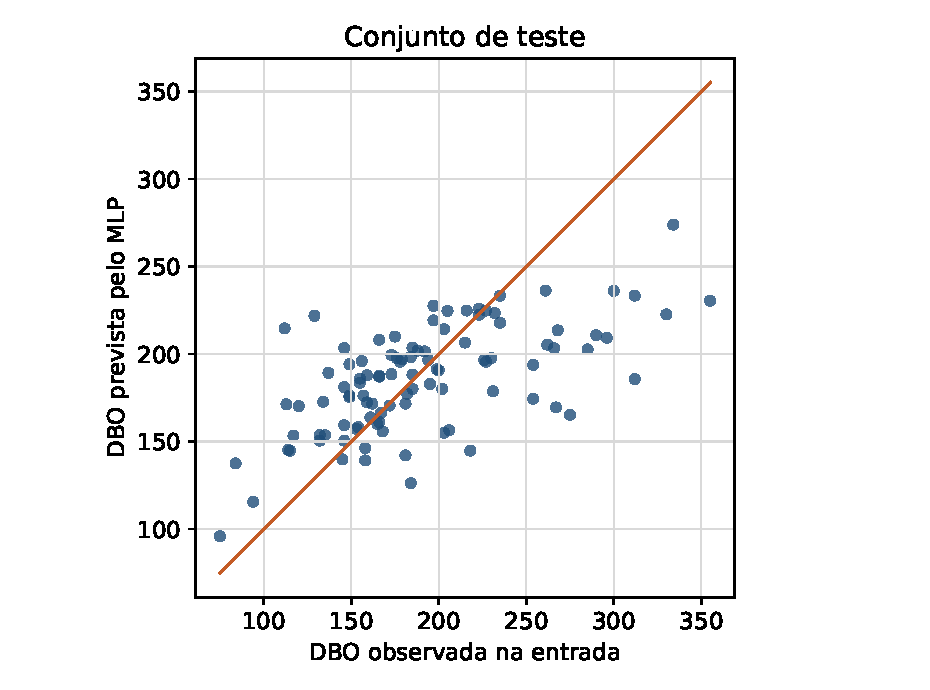
\includegraphics[width=0.78\textwidth]{figuras/observado_previsto.pdf}
\caption{Teste do MLP. A reta marca a previsão igual à DBO observada. Abaixo dela, a rede fica aquém da observação.}
\label{fig:previsto}
\end{figure}

\begin{figure}[H]
\centering
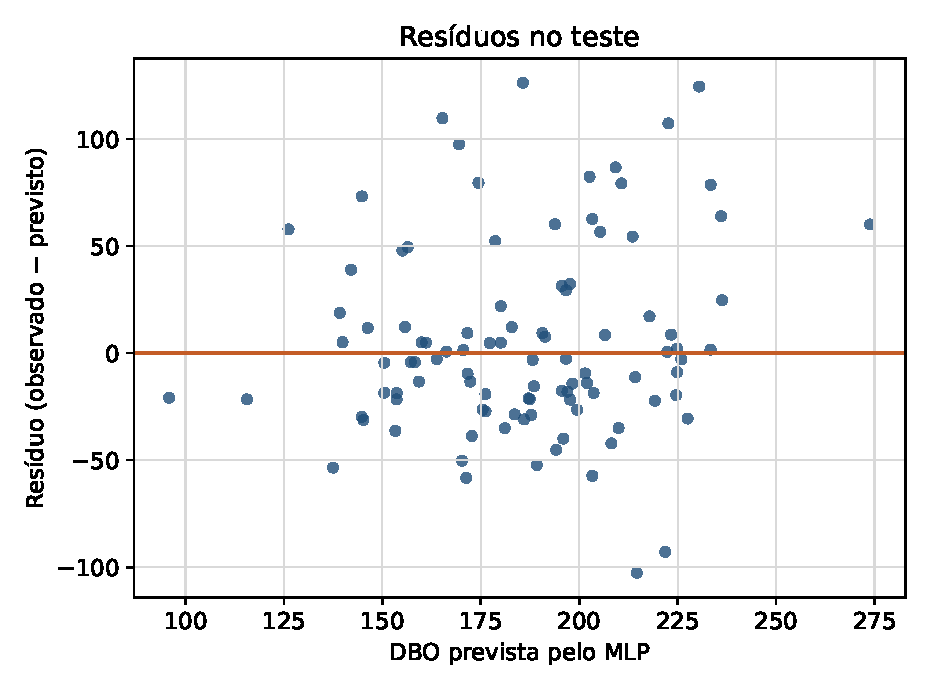
\includegraphics[width=0.78\textwidth]{figuras/residuos.pdf}
\caption{Resíduos no teste. A dispersão permanece larga em toda a faixa prevista.}
\label{fig:residuos}
\end{figure}

\begin{figure}[H]
\centering
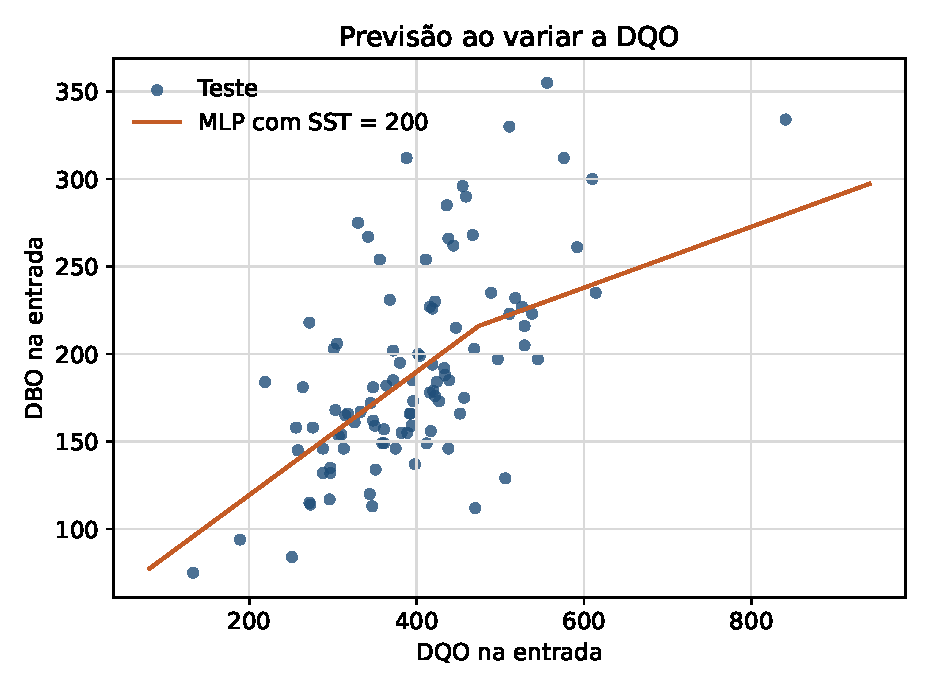
\includegraphics[width=0.78\textwidth]{figuras/dbo_por_dqo.pdf}
\caption{DBO e DQO no teste. A curva é o MLP com o SST fixo em 200, a mediana do treino.}
\label{fig:dqo}
\end{figure}

\section{Leitura}

O MLP reduz o MAE de 44,11 para 33,51 em relação a prever sempre a média do treino, cerca de um quarto a menos. O \(R^{2}\) de 0,37 deixa a maior parte da variação da DBO por explicar. O erro médio no teste equivale a cerca de 18\% da DBO média desse conjunto (191).

A mediana do erro, 22, é bem menor que o MAE, 33,5. Poucos dias puxam a média: um em cada dez erra 79 ou mais. O RMSE de 44,91, acima do MAE, descreve essa cauda.

A nuvem da Figura~\ref{fig:residuos} ocupa de cerca de \(-100\) a \(+130\) em qualquer região da previsão. Na Figura~\ref{fig:previsto}, DBO baixa fica acima da reta e DBO alta fica abaixo: a rede comprime os extremos. No teste a previsão vai até 274, enquanto várias observações passam disso e outras ficam abaixo de 100.

A curva da Figura~\ref{fig:dqo}, com SST fixo, é quase uma reta, com uma leve mudança de inclinação depois de DQO perto de 500, região com poucos dias. A regressão linear fica à frente do MLP por uma margem pequena, na validação cruzada e no teste. Com duas entradas e esta amostra, a rede de 8 neurônios reproduz uma relação praticamente linear. Redes maiores na grade ficam no mesmo patamar de erro.

O sinal útil está na DQO. O SST, mesmo com um valor extremo de 2008, deixa o MAE praticamente no mesmo lugar. Para este alvo e estas duas entradas, a descrição que cabe aos dados é a reta da equação anterior: a DBO prevista sobe cerca de 0,29 unidade por unidade de DQO.

A divisão trata os dias como independentes, que foi a regra desta análise. Dias vizinhos no calendário podem ter carga parecida; um teste cronológico, com o futuro separado do passado, pode dar erro maior do que o reportado aqui.

\section{Conclusão}

Com DQO e SST da entrada, o MLP chega a MAE 33,51, RMSE 44,91 e \(R^{2}\) 0,37 nos 100 dias de teste. A regressão linear chega a MAE 32,96, RMSE 44,76 e \(R^{2}\) 0,38, e também fica à frente na validação cruzada. A DQO carrega a estimativa. O SST fica sem efeito prático. O modelo acompanha o centro da DBO e se afasta nos dias extremos.

O notebook com o ajuste, a grade e os gráficos é \texttt{modelo/mlp\_dbo\_entrada.ipynb}.
\end{document}
